\appendix

% \subsection{Interference between TTFT and ITL in P/D Coupled Architecture}
% \label{subsubsec:pd-interference}

% \jiahuan{TODO}

% \begin{figure}[!ht]
%     \centering
%     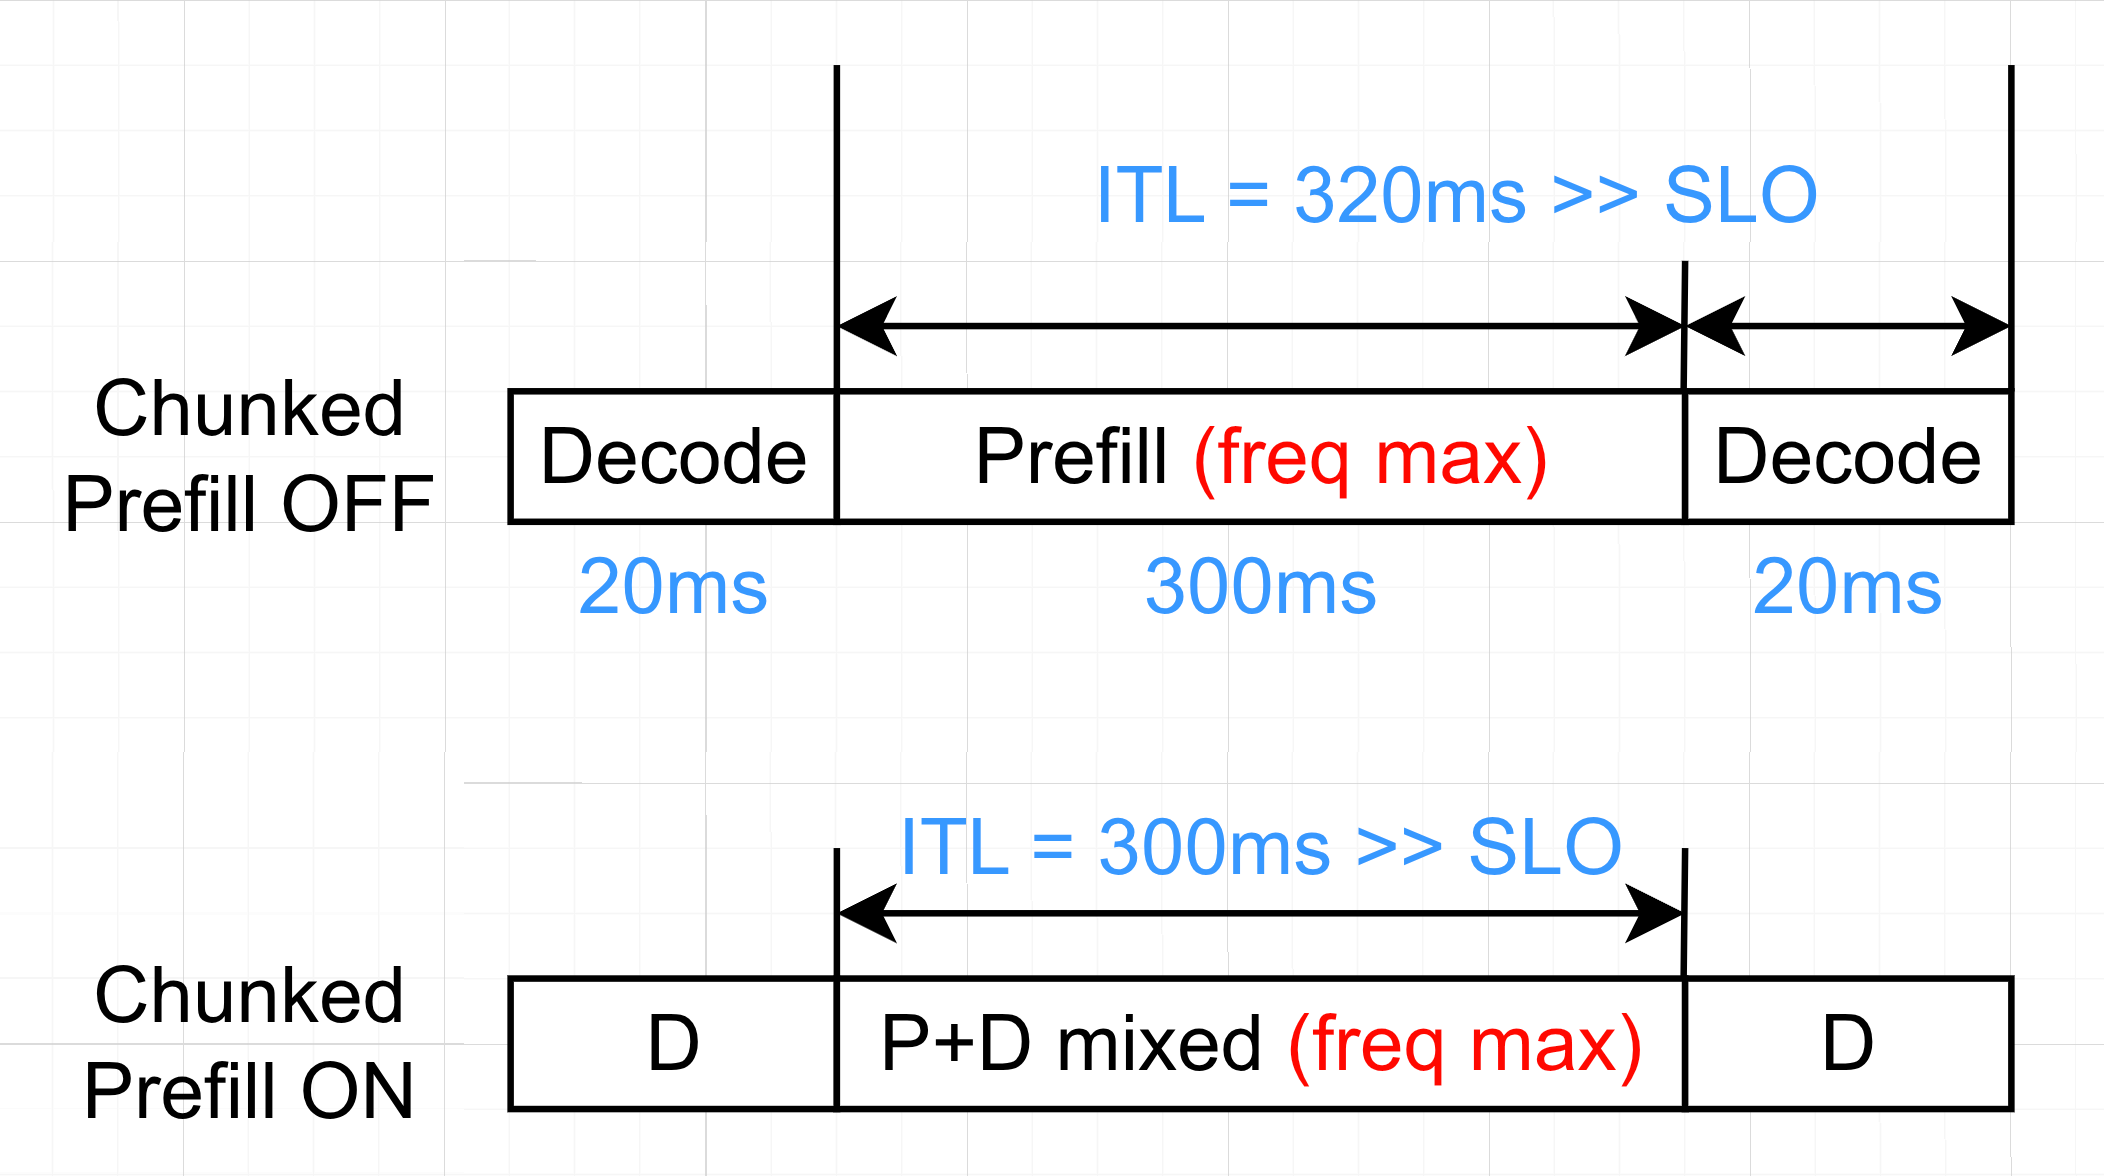
\includegraphics[width=\columnwidth]{figs/GetImage.png}
%     \caption{P/D interference on the collocated architecture.}
%     \label{fig:pd-collocated}
% \end{figure}


% \begin{figure}[!ht]
%     \centering
%     \includegraphics[width=\columnwidth]{example-image-a}
%     \caption{P/D interference on the collocated architecture.}
%     \label{fig:pd-collocated}
% \end{figure}

\subsection{Batch Size Boundaries of Prefill Phase}
\label{appendix:prefill-tile}

\fref{fig:ttft_vs_tokens-small}, a zoomed-in view of \fref{fig:pred-ttft}, focuses on the prefill phase with small numbers of batched tokens to show the relationship between prefill model inference time and batched token numbers ($N_{\text{tok}}$).
We can observe similar ``staircase-like'' tile effect like decode phase (\fref{fig:pred-itl}).
However, this effect only exist when batched token numbers are relative small.
When number of batched tokens goes over about 2000 (which is the dominate situation), this effect gradually becomes less significant.

\begin{figure}[!ht]
    \centering

    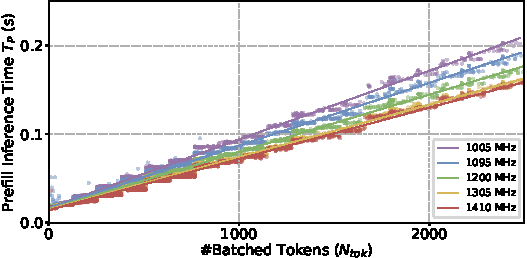
\includegraphics[width=\linewidth]{figs/ttft_vs_tokens-small.pdf}
    \caption{Zoomed-in version of \fref{fig:pred-ttft} for small batched token numbers: relationship between prefill model inference time and batched token numbers ($N_{\text{tok}}$) (LLaMA-3.1-8B on A100).}
    % \jiahuan{redraw}
    \label{fig:ttft_vs_tokens-small}
\end{figure}




% \subsection{Formal Algorithm of Frequency Selection in \governor}
% \label{subsubsec:freq-sel-algo}

% \aref{alg:ecofreq} gives a detailed formal version of frequency selection algorithm in \sref{subsec:governor}.
% Check texts in \sref{subsec:governor} to find text description of each step.

% \begin{algorithm}[!ht]
% % \caption{\governor: SLO-Aware and Iteration-Level Frequency Selection}
% \caption{\governor: SLO-Aware Frequency Selection}
% % \minjia{This algorithm only shows how to select frequency but it does not show how it performs control, e.g., where this control is placed? You may need to add the inference step loop and add the control right before the call of the decoding step.}
% % \jiahuan{my idea is, this is just the frequency selection algorithm, \fref{fig:governor-exec-flow} shows the control process. I believe it is more clear. Is it OK?}
% % \minjia{Yes.}
%  \label{alg:ecofreq}
%  \begin{algorithmic}[1]

%     \Require Current system status $\mathbf{M}$, batch information $\mathbf{B}$, frequency option list $\mathcal{F}$, model inference time predictors $T_P(\cdot)$ and $T_D(\cdot)$, TTFT SLO $S_P$, ITL SLO $S_D$.
    
%     \Ensure Selected GPU frequency $f$.

%     \If{$\Call{HasWaitingReqs}{\mathbf{M}}$}  \Comment{\textbf{step \ding{202} Queue check}} \label{algline:step1-beg}
%         \State \Return $\max(\mathcal{F})$ \Comment{clear backlogged reqs timely}
%     \EndIf \label{algline:step1-end}

%     \If{$\Call{IsPrefill}{\mathbf{B}}$} \Comment{\textbf{step \ding{203} Phase adjustment}} \label{algline:step2-beg}
%         \Statex /* prefill: deduct the waiting time from SLO budget */
%         \State $S \gets S_P - \max( \mathbf{T}_{\text{waiting}}(\mathbf{B}) )$, $T_{\text{inference}}(\cdot) \gets T_P(\cdot)$ 
%         % \State $T_{\text{inference}}(\cdot) \gets T_P(\cdot)$
%     \Else
%         \State $S \gets S_D$, $T_{\text{inference}}(\cdot) \gets T_D(\cdot)$ \Comment{/* decode */}
%     \EndIf \label{algline:step2-end}

%     % \State $f^\star = \argmin_{f\in\mathcal{F}} T_{\text{inference}}(\mathbf{M}, \mathbf{B}, f) \le S$
%     % \If 

%     % \State $f^\star = \argmin_{f\in\mathcal{F}} T_{\text{inference}}(\mathbf{M}, \mathbf{B}, f) \le S$ \Comment{\textbf{step \ding{204} Frequency selection}} \label{algline:step3-beg}
%     % \If{$f^\star \ne \emptyset$} 
%     %     \State $f^\star = \max(\mathcal{F})$ \Comment{no freq can meet SLO, return max}
%     % \EndIf
    

%     \For{$f \in \sorted(\mathcal{F})$}  \Comment{\textbf{step \ding{204} Frequency selection}} \label{algline:step3-beg}
%         \If{$T_{\text{inference}}(\mathbf{M}, \mathbf{B}, f) \le S$}
%             \State \Return $f$ \Comment{minimum frequency to meet the SLO}
%         \EndIf
%     \EndFor

%     \State \Return $\max(\mathcal{F})$  \Comment{no freq can meet SLO, return max} \label{algline:step3-end}

%  \end{algorithmic}
% \end{algorithm}



\subsection{Formal Routing Algorithm Description of \router}
\label{subsubsec:router-algo-blk}

\aref{alg:ecoroute} provides a detailed formal version of routing algorithm proposed in \sref{subsec:router}.
Check \sref{subsec:router} for text description of each step.

\begin{algorithm}[!ht]
 \caption{\router: Decode Request Routing}
 \label{alg:ecoroute}
 \begin{algorithmic}[1]

    \Require Decode instance list $\mathcal{D}=\{d_i\}_{i=1}^n$ and their state list $\mathcal{M}=\{m_i\}_{i=1}^n$, request for routing $r$, frequency decision of \governor $\freq(\cdot)$, frequency threshold $\Delta$.

    \Ensure Selected decode instance $d\in\mathcal{D}$.

    \State $\mathcal{F} \gets \{ \freq(m_i)\}_{i=1}^n$ \Comment{current freq of all instances}
    \State $\mathcal{F}^\prime \gets \{ \freq(m_i \oplus r)\}_{i=1}^n$ \Comment{frequency after hypothetically adding request $r$, $\oplus$ denotes adding request}

    \If{\Call{PartialChanged}{$\mathcal{F}$, $\mathcal{F}^\prime$} $\And$ $\max(\mathcal{F}^\prime)-\min(\mathcal{F}^\prime) \le \Delta$}
        \Statex /* \textbf{case} \ding{202}: if some but not all instances change the frequency, and the frequency difference $\le$ threshold */
        \State \Return $d_{\argmin_i \Call{Unchanged}{\mathcal{F}, \mathcal{F}^\prime}}$ \Comment{min unchanged}
    \EndIf
    \Statex /* \textbf{case} \ding{203}: other situations */
    \State \Return \Call{RoundRobin}{$d_{\argmin_i \mathcal{F}^\prime}$} \Comment{round-robin of min}

    % \If{$\mathcal{F}=\mathcal{F}^\prime$} \Comment{\textbf{case \ding{202}}: no frequency changes}
    %     \If{\Call{AllSame}{$\mathcal{F}$}} \Comment{\textbf{\ding{202}(a)}: all freqs are same}
    %         \State \Return \Call{RoundRobin}{$\mathcal{D}$} \Comment{round-robin}
    %     \Else  \Comment{\textbf{\ding{202}(b)}: not all same}
    %         \State \Return $d_{\argmin_i \mathcal{F}}$ \Comment{min current freq}
    %     \EndIf
    % \ElsIf{\Call{PartialChanged}{$\mathcal{F}$, $\mathcal{F}^\prime$}} \Comment{\textbf{case \ding{203}}: some frequencies increase}
    %     \If{$\max(\mathcal{F}^\prime)-\min(\mathcal{F}^\prime) \le \Delta$}  \Comment{\textbf{\ding{203}(a)}: diff $\le\Delta$}
    %         \State \Return $d_{\argmin_i \Call{Unchanged}{\mathcal{F}, \mathcal{F}^\prime}}$ \Comment{min unchanged}
    %     \Else  \Comment{\textbf{\ding{203}(b)}: diff $>\Delta$}
    %         \State \Return $d_{\argmin_i \mathcal{F}^\prime}$ \Comment{min resulting freq}
    %     \EndIf
    % \EndIf
    % \State \Return $d_{\argmin_i \mathcal{F}^\prime}$  \Comment{\textbf{case \ding{204}}: all frequency increase}
    % \Else \Comment{\textbf{case \ding{204}}: all frequencies increase}
    %     \State \Return $d_{\argmin_i \mathcal{F}^\prime}$ \Comment{min resulting freq}
    % \EndIf

 \end{algorithmic}
\end{algorithm}

\subsection{XGBoost Configuration of \predictor}
\label{subsubssec:xgboost}

As discussed in \sref{subsec:predictor}, we employ XGBoost~\cite{chen2016xgboost} to predict prefill and decode model inference times based on system states and batch information.
The model configuration details are as follows:
\begin{lstlisting}
import xgboost as xgb

# prefill model
model_prefill = xgb.XGBRegressor(
    objective="reg:absoluteerror",
    n_estimators=100000,
    learning_rate=0.5,
    booster='gblinear',
    max_depth=6,
    subsample=0.8,
    colsample_bytree=0.8,
    tree_method='hist',
    random_state=42,
    eval_metric='mae',
    early_stopping_rounds=1000,
)

# decode model
model_decode = xgb.XGBRegressor(
    objective="reg:absoluteerror",
    n_estimators=1000,
    learning_rate=0.1,
    booster='gbtree',
    max_depth=6,
    subsample=0.8,
    colsample_bytree=0.8,
    tree_method='hist',
    random_state=42,
    eval_metric='mae',
    early_stopping_rounds=200,
)
\end{lstlisting}



\subsection{Length Distribution of ShareGPT and LMSYS Dataset}
\label{appendix:dataset-length}

\tref{tab:length_statistics} summarizes the statistical properties of the ShareGPT and LMSYS datasets used in the evaluation, including the mean and standard deviation of their input and output lengths.
The cumulative distribution functions (CDFs) for these length distributions are visualized in \fref{fig:dataset-distribution}.
Analysis of this data shows that:


\begin{itemize}
    \item ShareGPT has longer prefill and decode length compared to LMSYS dataset.
    \item ShareGPT has larger prefill/decode length ratio.
\end{itemize}

\begin{figure}[!ht]
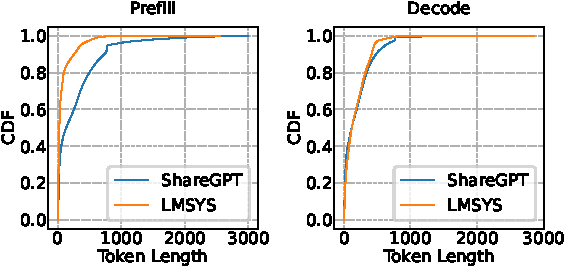
\includegraphics[width=\linewidth]{figs/cdf_plot.pdf}
    \caption{CDF of prefill and decode lengths for the ShareGPT and LMSYS datasets.}
    \label{fig:dataset-distribution}
\end{figure}


\begin{table}[!ht]
    \centering
    \caption{Length distribution of datasets used in our evaluation. Std refers to standard deviation.}
    \label{tab:length_statistics}
    \begin{tabularx}{\columnwidth}{C | C C C C}
        \toprule
        \textbf{Dataset} & \multicolumn{2}{c}{\textbf{Prefill}} & \multicolumn{2}{c}{\textbf{Decode}} \\
        \cmidrule(lr){2-3} \cmidrule(lr){4-5}
        & \textbf{Mean (ms)} & \textbf{Std (ms)} & \textbf{Mean (ms)} & \textbf{Std (ms)} \\
        \midrule
        ShareGPT & 280.27 & 375.58 & 190.90 & 209.15 \\
        LMSYS    & 78.40  & 133.29 & 174.57 & 166.13 \\
        \bottomrule
    \end{tabularx}
    % \begin{tabular}{c|cccc}

    % \end{tabular}
\end{table}




\subsection{Extra Throughput Data of The Main Result}
\label{subsubsec:ablation-throughput}

We compute the throughput from the experimental results in \sref{subsec:main-result} using ShareGPT dataset on LLaMA-3.1-8B.
As shown in \fref{fig:throughput}, \name achieves slightly lower throughput than SGLang with static maximum frequency due to its opportunistic frequency scaling, but not at the cost of SLO violations.
Furthermore, at high request rates where greater throughput is required, \name can also adaptively achieve nearly the same throughput as SGLang with static maximum frequency.

\begin{figure}[!ht]
    \centering
    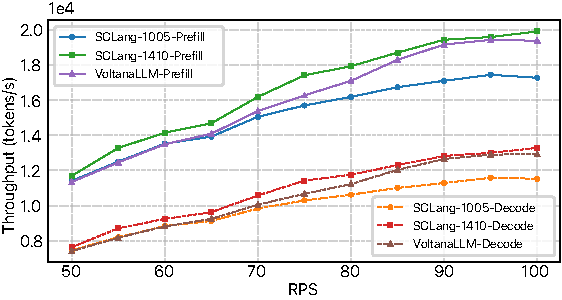
\includegraphics[width=\linewidth]{figs/throughput.pdf}
    \caption{Comparing throughput of \name with baselines for LLaMA-3.1-8B and ShareGPT dataset.}
    \label{fig:throughput}
\end{figure}



\subsection{Extra TTFT and ITL CDFs of The Main Result}
\label{subsubssec:main-cdf}

\fref{fig:main-cdf} shows the TTFT and ITL CDFs corresponding to the results in \sref{subsec:main-result}.
The figure provides CDFs across all model and dataset combinations (organized by column).
For each combination, CDFs are presented for both low request arrival rates (rows 1 and 3) and high request rates (rows 2 and 4).
The results show that when the request arrival rate is low, \name achieves latency CDFs similar to SGLang-1005, as the low frequency is sufficient for SLO attainment.
In contrast, when the request rate is high, \name adaptively increases its frequency, achieving latency CDFs similar to SGLang-1410.


\cameraready{

\subsection{Comparison with More Intermediate Static Frequency Baselines}
\label{subsubsec:intermidate-static-freq}


To evaluate whether intermediate static frequencies can achieve similar efficiency benefits, we compare \name against SGLang operating at fixed intermediate frequencies of 1095~MHz, 1200~MHz, and 1305~MHz, using LLaMA-3.1-8B model and ShareGPT dataset.
As \fref{fig:intermidate-static-freq} shows, because these static configurations inherently lack dynamic adaptability, they consistently consume significantly more energy than \name at low request rates.
Conversely, at high RPS, these static intermediate frequencies fail to provide the necessary compute throughput, which degrades SLO attainment compared to \name.
This confirms that static frequency tuning, regardless of the specific frequency chosen, is insufficient for energy-efficient, SLO-aware frequency control.

\begin{figure}[!ht]
    \centering
    
\includegraphics[width=\columnwidth]{figs_extra/figure_1_multi_freq.pdf}
    \caption{Comparison of energy consumption and SLO attainment between \name and SGLang with intermediate static frequencies across varying request rates, using LLaMA-3.1-8B model and ShareGPT dataset.}
    \label{fig:intermidate-static-freq}
\end{figure}


\subsection{Comparison with Power-Capped Baselines}
\label{subsubsec:power-capped}

We also evaluate \name against power-capped baselines.
Fundamentally, power-capping acts as an indirect upper-bound on frequency, rather than a responsive alternative to our per-engine-iteration frequency control.
We evaluate a 350W statically-capped SGLang configuration against the default 400W limitation, using LLaMA-3.1-8B model and ShareGPT dataset.
Our results in \fref{fig:power-capped} demonstrate that power-capping lacks adaptability for workload dynamism.
Specifically, at low request rates, the power-capped baseline fails to optimally lower frequencies, thus consuming substantially more energy than \name for similar SLO attainment.
Furthermore, at high RPS, the power cap strictly prevents the system from boosting frequency when necessary, which inherently degrades overall SLO attainment.

\begin{figure}[!ht]
    \centering
    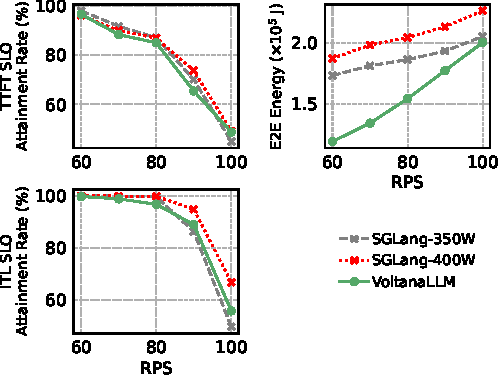
\includegraphics[width=\columnwidth]{figs_extra/figure_2_power_capped.pdf}
    \caption{Comparison of energy consumption and SLO attainment between \name and a 350W power-capped SGLang across varying request rates, using LLaMA-3.1-8B model and ShareGPT dataset.}
    \label{fig:power-capped}
\end{figure}


\subsection{Detailed Phase-Specific Energy Gain}
\label{subsubsec:phase-specific-energy-gain}

To understand where our solution brings the most gain within the disaggregated architecture, we decompose the energy savings from the configuration LLaMA-3.1-8B@ShareGPT in \sref{subsec:eval-method} into the prefill and decode phases.
As \fref{fig:phase-specific-energy-gain} shows, the benefits are load-dependent.
At low request rates, the decode phase yields greater energy savings, which is attributed to its inherently lower arithmetic intensity.
Conversely, at high RPS, the prefill phase contributes more significantly to the overall energy savings. This shift occurs because our \governor effectively exploits short-term, low-load durations within the prefill phase to perform iteration-level frequency reductions, whereas the decode instances must remain at higher frequencies to satisfy strict ITL SLOs under heavy load.

\begin{figure}[!ht]
    \centering
    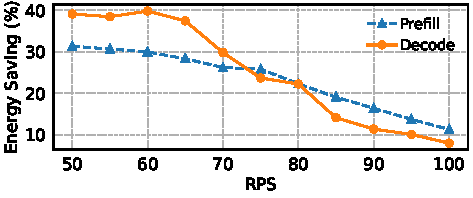
\includegraphics[width=\columnwidth]{figs_extra/figure_3_phase_specific.pdf}
    \caption{Energy saving percentage of each phase for \name under the LLaMA-3.1-8B@ShareGPT configuration in \sref{subsec:eval-method}.}
    \label{fig:phase-specific-energy-gain}
\end{figure}

}


\subsection{Do More Frequency Levels Bring Benefits?}
\label{subsubsec:exp-multi-level}


In \sref{subsec:main-result}, \name is configured with two-level frequency options.
To analyze the potential benefits of finer-grained levels, we extend \governor's frequency options to five levels: $\mathcal{F}=\{1005, 1095, 1200, 1305, 1410\}$ MHz, and evaluate it using the ShareGPT dataset on LLaMA-3.1-8B, following the same settings as \sref{subsec:main-result}.
\fref{fig:freq-level} presents the results.
For prefill, finer frequency granularity yields negligible benefits, as the significant iteration-level workload variation (\fref{fig:prefill-tokens-fluctuation}) makes the middle levels largely unused.
In contrast, the decode reveals a trade-off: finer granularity offers slight energy savings but at the cost of lower SLO attainment rates.
This allows users to select appropriate granularities based on their specific performance-energy priorities.


\begin{figure}[!ht]
    \centering
    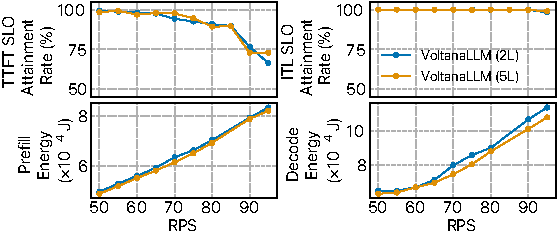
\includegraphics[width=\columnwidth]{figs/ablation_multilevel_tr.pdf}
    \caption{Comparison of \name with different frequency levels. \name (2L) uses two frequency levels, while \name (5L) uses five. Both configurations maintain similar TTFT/ITL attainment and energy trends when combined with \router.}
    % \jiahuan{@Junfeng, change the y axis label of 2nd row to 3 lines}

    \label{fig:freq-level}
\end{figure}



\cameraready{

\subsection{Sensitivity Analysis of $\Delta$ in \router}
\label{subsubsec:delta-analysis}

As discussed in \sref{subsec:router}, $\Delta$ serves as a guardrail against extreme workload imbalance, where a smaller value indicates a stricter tolerance.
While $\Delta$ remains largely inactive for 2-level frequency configurations where the frequency gap is a deliberate design target, it becomes crucial in multi-level frequency settings (e.g., 5-level configurations).
In these scenarios, $\Delta$ constrains the frequency variance between instances, preventing \governor from over-allocating requests to high-frequency instances while leaving lower-frequency instances underutilized.

To evaluate the sensitivity and robustness of \router to the frequency spread threshold $\Delta$, we set \name across $\Delta \in \{110, 210, 310, 410\}$, with 5-level frequencies $\mathcal{F}=\{1005, 1095, 1200, 1305, 1410\}$ MHz in \governor.
Other settings follow \appref{subsubsec:exp-multi-level}.
Our results shown in \fref{fig:delta-analysis} indicate that while larger $\Delta$ values can slightly degrade ITL SLO attainment at high RPS due to imbalance, the choice of $\Delta$ is generally robust, with all tested values delivering stable and comparable performance.

\begin{figure}[!ht]
    \centering
    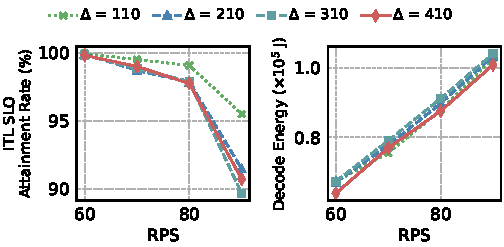
\includegraphics[width=\columnwidth]{figs_extra/figure_4_delta.pdf}
    \caption{Impact of $\Delta \in \{110, 210, 310, 410\}$ on ITL SLO attainment and energy performance under 5-level frequency setting.}
    \label{fig:delta-analysis}
\end{figure}

}






\subsection{An Example of Comparison between Round-Robin and \router}
\label{subsubsec:router-example}

\fref{fig:bs-time} compares round-robin and \router by the batch size and frequencies of the two decode instances over time.
\fref{fig:router-example} in \sref{subsec:router} is a conceptual version of it.
It shows \router can restrict the batch size of one instance under a specific boundary (256) so it can operate at a lower frequency.
That is a good example to show how \router save energy by avoiding frequency ``cliff'' discussed in \fref{fig:router-motivation}.

\begin{figure}[!ht]
    \centering
    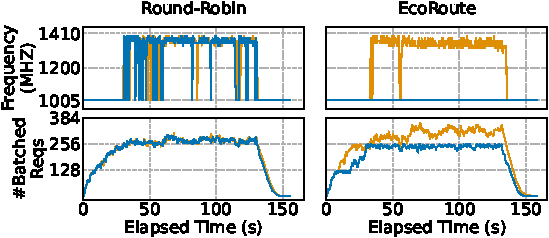
\includegraphics[width=\columnwidth]{figs/ablation-router.pdf}
    \caption{An example of how \router differs from round-robin policy (RPS=75). Each line represents a decode instance. \router keeps one instance below the batch size boundary (256), allowing it to run at a lower frequency for longer time. }    
    % \minjia{Candidate move to the appendix.}
    % \jiahuan{if we decide to remove this figure from here, can we replace \fref{fig:router-example} with this figure. \fref{fig:router-example} is just a conceptual version of it.}
    % \minjia{Yes, although I would try to avoid adding too many empirical results in the design. }
    \label{fig:bs-time}
\end{figure}







\subsection{U-Shape Figures of GH200}
\label{subsubssec:u-shape-gh200}

\fref{fig:u-shape-gh200} illustrates the U-shaped energy-frequency curves and monotonically decreasing latency-frequency curves when serving Qwen3-32B~\cite{yang2025qwen3} on a GH200.
These results exhibit trends similar to those of the A100 (\fref{fig:u-shape}), but with distinct hardware-specific differences.
The prefill phase remains power-intensive, hitting the GH200's 900W TDP limitation at $\approx$1600 MHz. Furthermore, the two phases possess different energy sweet spots: the optimal point for prefill is $\approx$1095 MHz, while for decode, it is $\approx$1395 MHz.

\begin{figure}[!ht]
    \centering
    \begin{subfigure}[b]{0.49\columnwidth}
        \centering
        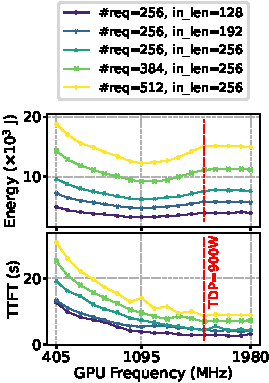
\includegraphics[width=\linewidth]{figs/prefill_energy_ttft_gh200.pdf}
        \caption{Prefill phase.}
    \end{subfigure}
    \hfill
    \begin{subfigure}[b]{0.49\columnwidth}
        \centering
        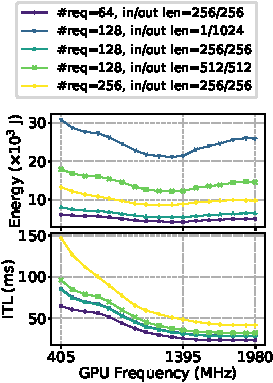
\includegraphics[width=\linewidth]{figs/decode_energy_itl_gh200.pdf}
        \caption{Decode phase.}
    \end{subfigure}
    \caption{Impact of GPU frequency on energy (up) and latency (down) for P/D phases on GH200 with Qwen3-32B. Prefill hits TDP limitations (900 W) near 1600 MHz.
    Both phases exhibit U-shaped energy-frequency curves, but prefill reach energy sweet spot $\approx$1095 MHz, while decode reach energy sweet spot $\approx$1395 MHz.}
    \label{fig:u-shape-gh200}
    % \begin{subfigure}[b]{0.49\columnwidth}
    %     \centering
    %     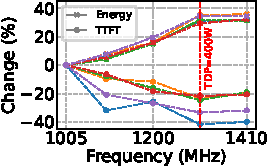
\includegraphics[width=\linewidth]{figs/prefill_energy_ttft_pct.pdf}
    %     \caption{Prefill phase.}
    %     \label{fig:u-shape-p}
    % \end{subfigure}
    % \hfill
    % \begin{subfigure}[b]{0.49\columnwidth}
    %     \centering
    %     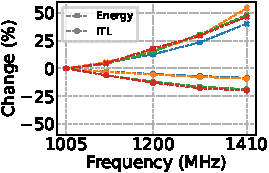
\includegraphics[width=\linewidth]{figs/decode_energy_itl_pct.pdf}
    %     \caption{Decode phase.}
    %     \label{fig:u-shape-d}
    % \end{subfigure}

    % \caption{Impact of GPU frequency on energy and latency (TTFT/ITL) for P/D phases. Both phases exhibit U-shaped energy-frequency curves but differ significantly in sensitivity: prefill is compute-bound and TDP-limited near 1305 MHz, whereas decode is often memory-bound and yields only $\approx$20\% ITL reduction for $\approx$50\% higher energy. These phase-specific trade-offs motivate independent and adaptive frequency control. \jiahuan{TODO (as reviewer suggests) extend to all frequencies for the lower figures.}}
    % \label{fig:u-shape}
\end{figure}






\subsection{What happens in varying the P/D throughput demand ratio?}
\label{subsubsec:ablation-pd-ratio}


As discussed in \sref{subsec:temporal-variation}, the temporal variation of P/D throughput demand ratio requires phase-specific frequency control.
However, evaluating the whole Azure LLM Inference Trace dataset incurs significant GPU cost and time given it only shows fluctuation on the scale of hours.
Hence, we use a synthetic dataset with P/D demand ratio fluctuating in 5 minutes.
\fref{fig:ablation-pd-ratio} shows the evaluation results with LLaMA-3.1-8B using the same configuration in \sref{subsec:main-result}.

The results shown in \tref{tab:ablation-pd-ratio} confirm the adaptiveness of \name.
It can still maintain comparable SLO attainment rates to SGLang at maximum frequency, while obtain significant energy savings.
\fref{fig:ablation-pd-ratio} shows the frequency dynamics.
When prefill throughput demand is high, the prefill instance operates at a higher frequency, while the decode instance remains at a low frequency.
Conversely, when decode throughput demand is high, the decode instance operates at a higher frequency, while the prefill instance remains at a low frequency.

\begin{figure}[!ht]
    \centering
    \begin{subfigure}[t]{0.42\columnwidth}
        \centering
        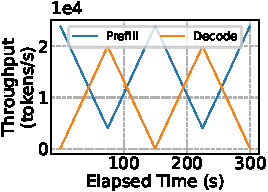
\includegraphics[width=\linewidth]{figs/ablation-pd-ratio-b.pdf}
    \end{subfigure}
    \hfill
    \begin{subfigure}[t]{0.53\columnwidth}
        \centering
        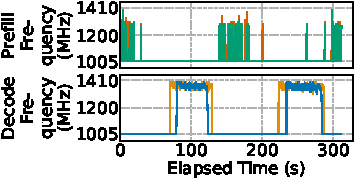
\includegraphics[width=\linewidth]{figs/ablation-pd-ratio-a.pdf}
    \end{subfigure}
    \caption{Left: P/D throughput with our synthetic dataset. Right: frequency dynamics of all instances in \name.}
    \label{fig:ablation-pd-ratio}
\end{figure}

\begin{table}[!ht]
    \centering
    \caption{Latency SLO attainment and end-to-end (E2E) energy consumption under a synthetic workload with varying P/D demand ratios.}
    \label{tab:ablation-pd-ratio}
    \begin{tabularx}{\columnwidth}{C | C C C}
        \toprule
        \textbf{Metrics} & TTFT SLO Attainment Rate (\%) & ITL SLO Attainment Rate (\%) &  E2E Energy (J) \\
        \midrule
        \textbf{\name} &96.05 &  91.74 & 289409\\
        \textbf{SGLang-1005} &77.86 & 36.78 & 257768 \\
        \textbf{SGLang-1410} &97.85 & 88.92 & 405340\\
        \bottomrule
    \end{tabularx}
\end{table}


\begin{figure*}[!ht]
    \centering
    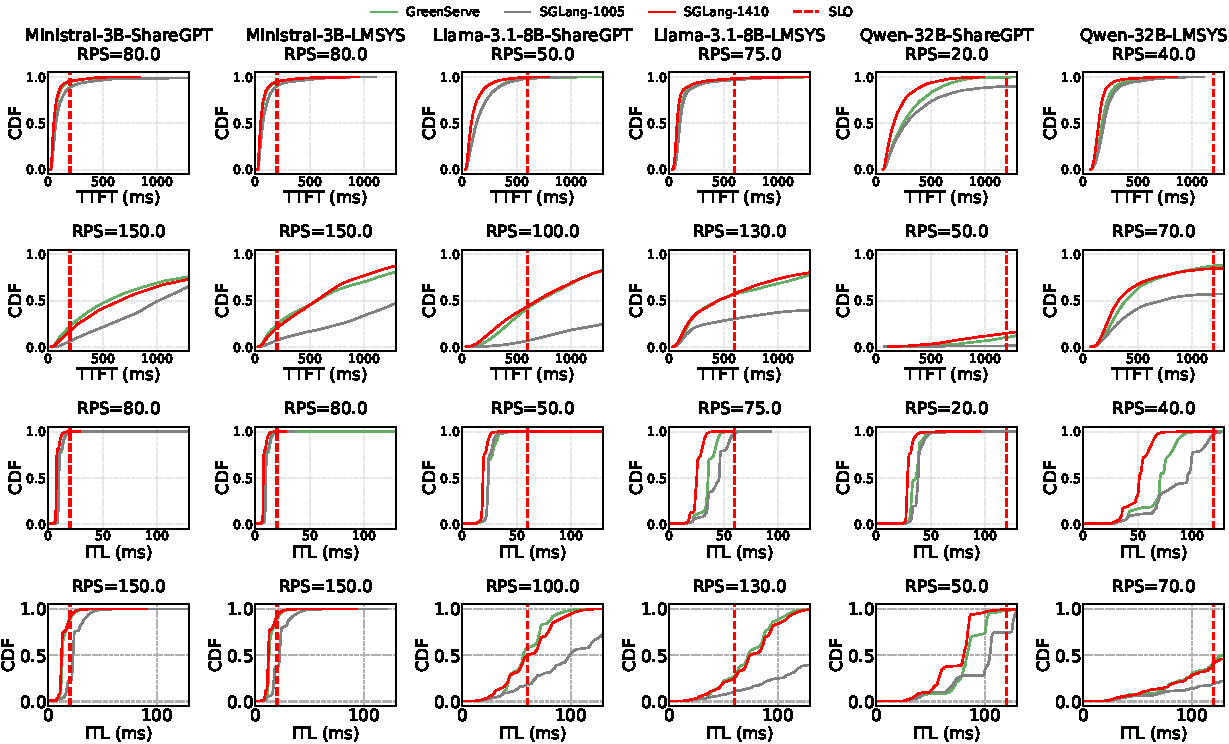
\includegraphics[width=0.95\linewidth]{figs/cdf.pdf}
    \caption{CDF of TTFT (top 2 rows) and ITL (bottom 2 rows) across various models and datasets (each column). For each model and dataset combination, we pick the smallest (row 1 and 3) and the largest (row 2 and 4) request arrival rates to shows the distinct behavior of \name under different workloads. Data comes from \fref{fig:main-result}.}
    % \jiahuan{@Junfeng, fix the font size as \fref{fig:main-result}. fix legend text and ciolor. Make sure they are consistent with \fref{fig:main-result}}
    \label{fig:main-cdf}
\end{figure*}